\documentclass[border=5pt]{standalone}
\usepackage{mathtools, pgfplots}
\DeclarePairedDelimiter\abs{\lvert}{\rvert}%
\DeclarePairedDelimiter\norm{\lVert}{\rVert}%

\pgfkeys{/pgfplots/Delta Style/.style={
    % scale only axis,
    % grid=major,
    axis equal,
    grid style={dashed, gray!30}, %Uncomment these lines for no grid
    axis lines=middle,
    inner axis line style={=stealth}, %Arrow type
    ultra thick,
    xlabel={\large $x$},
    ylabel={\large $y$},
    cycle list = {black,black!70,black!40,black!10} %Plot colors cycle in grayscale
  }}


\begin{document}
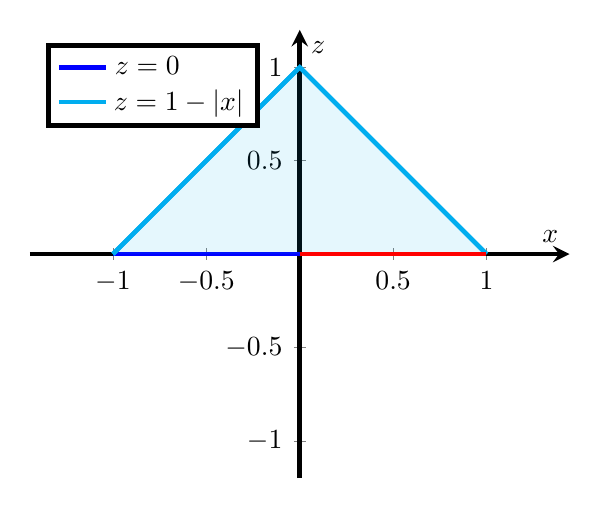
\begin{tikzpicture}
  \begin{axis}[Delta Style, xlabel = {$x$}, ylabel = {$z$}, 
    domain = -1:1,
    ymax = 1.2, ymin = -1.2,legend pos=north west]
    % Below the red parabola is defined
    \addplot [blue,domain=-1:0] {0}; \addlegendentry{$z=0\phantom{33.33}$}

    % Here the blue parabloa is defined
    \addplot [color=cyan,
              fill = cyan, fill opacity = 0.1, domain = -1:1] {1-abs(x)};
    
    \addplot [ color=cyan, fill = cyan, fill opacity = 0.1, domain = -1:0, ]
    {1+x};
 
    \addplot [ color=cyan, fill = gray, fill opacity = 0.1, domain = 0:1, ]
    {1-x}; \addlegendentry{$z=1 - \abs{x}$}
    \addplot [red,domain=0:1] {0}; 
  \end{axis}
\end{tikzpicture}
\end{document}
